
\begin{Q}
\textbf{\Large Expectation Maximization}

In this question, we expect you to do some computation related to the EM algorithm covered in the lecture.

\textbf{Background.} On the xy-plane, we have a rigid object, and our sensor can capture $N$ key points, whose coordinates are: $\mathcal{P}=\{\vp^{(1)}, \vp^{(2)}, ..., \vp^{(N)}\}$. ($N$ is a sufficiently large integer.) An unknown force then cause a translation $\mathbf{T}$ to this object, where $\mathbf{T}$ is encoded $T_x$ and $T_y$, meaning how long the object has moved along the x-axis and y-axis. To calculate parameter $\mathbf{T}$, we use our sensor to capture the key points on the rigid object one more time, acquiring a set of $N$ key points: $\mathcal{Q}=\{\vq^{(1)}, \vq^{(2)}, ..., \vq^{(N)}\}$. (See Fig.~\ref{fig:em} for an intuitive demonstration. The ``L'' is our rigid body, $N=3$, and the blue and red dots are the key points.)

\textbf{Assumption.} During this process, we assume that an bi-jection mapping between $\mathcal{P}$ and $\mathcal{Q}$ exists (See Fig.~\ref{fig:em}, the key points are all the corners of ``L.'') However, this bijection mapping cannot be directly got from the sensors, as the orders of the points may be shuffled during perception. 

\begin{figure}[h]
    \centering
    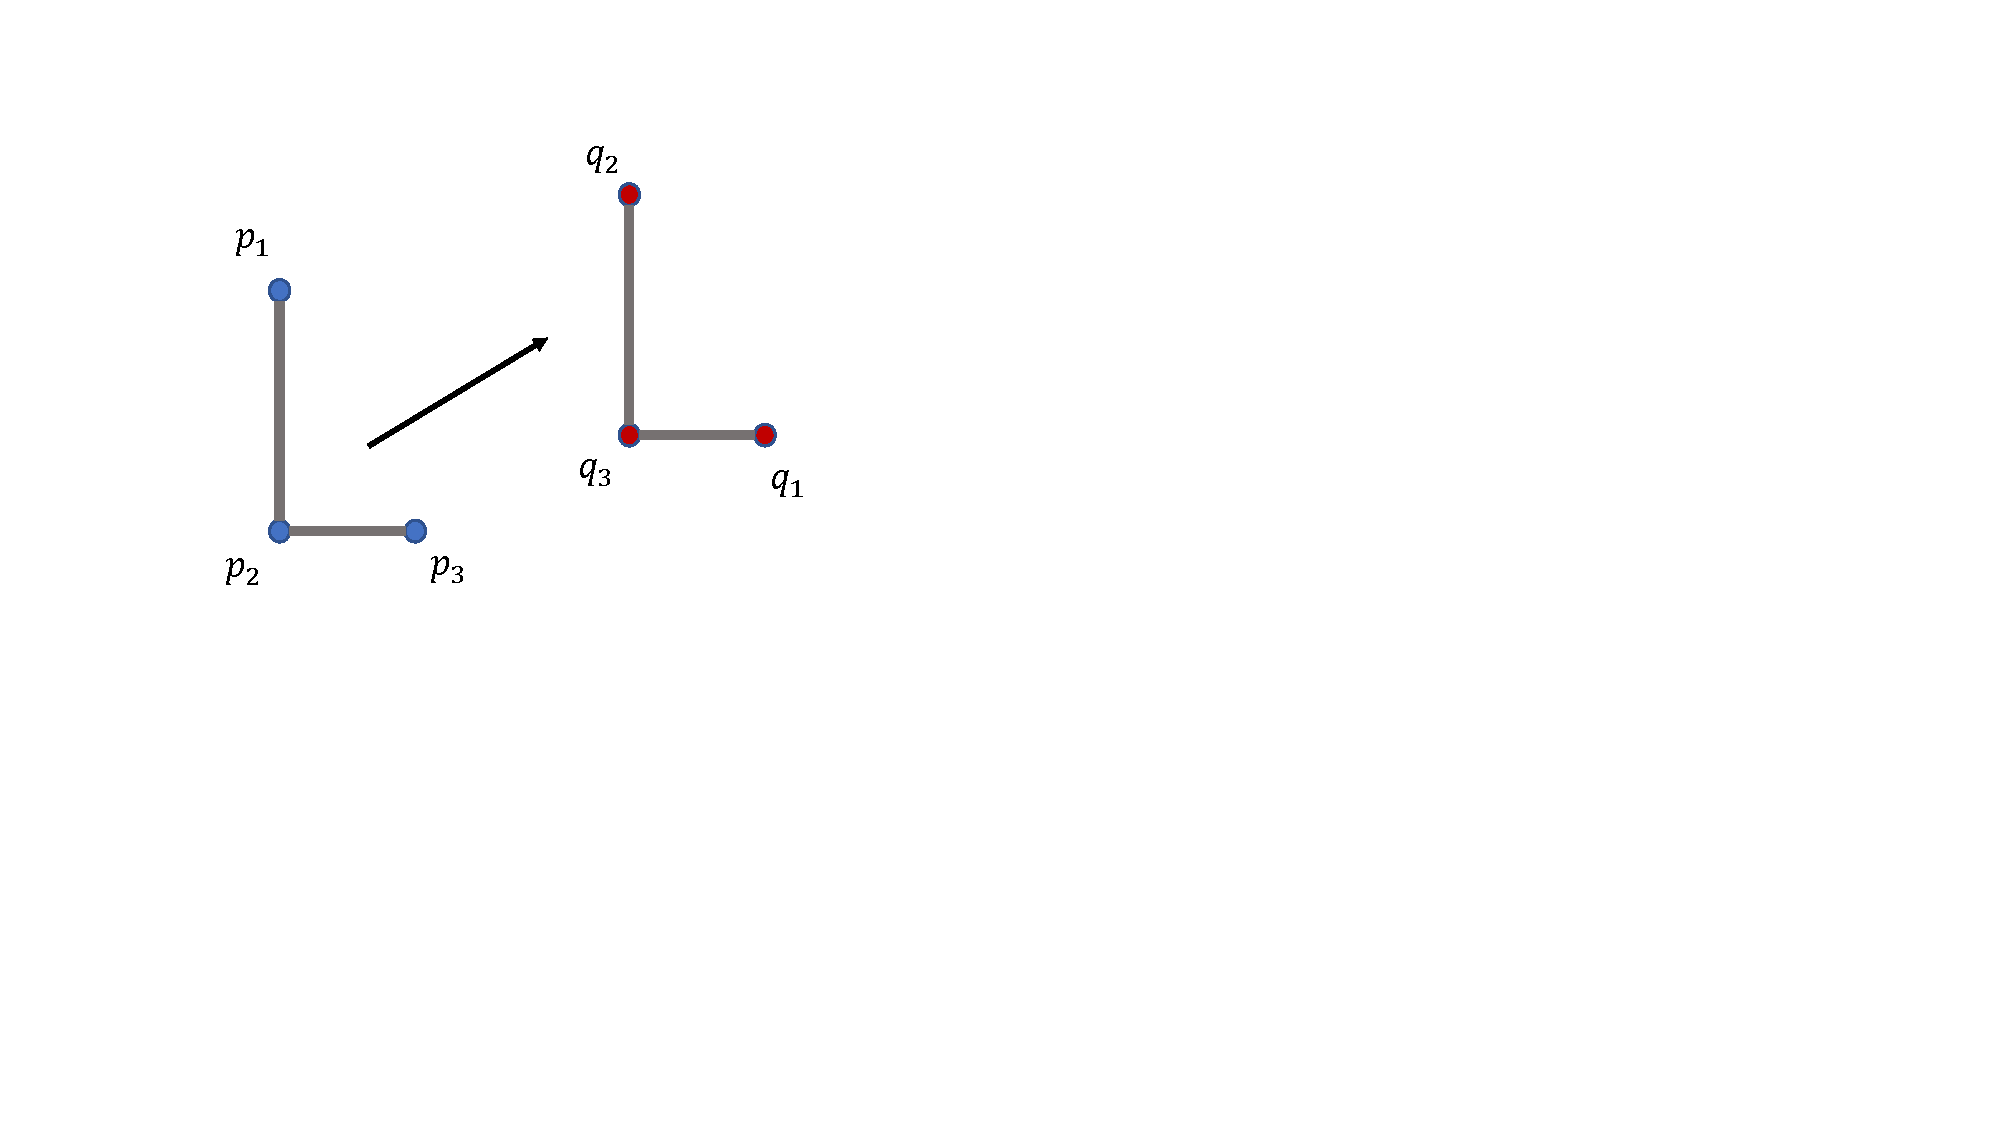
\includegraphics[width=0.6\columnwidth]{figs/em.pdf}
    \caption{}
    \label{fig:em}
\end{figure}

\textbf{Objective.} Using EM algorithm to estimate the translation parameter and the corresponding pairs of ke points, by introducing binary hidden variables $\vZ \in \mathbb{R}^{N\times N}$, where $Z_{ij}=1$ means  $\vp^{(i)}$ and $\vq^{(j)}$ are a match.

\textbf{Remark.} We have the following remarks on this question.

\begin{itemize}[itemsep=-1mm]
    \item This questions set is for you to understand the process of EM with an intuitive example without annoying mathematical equations. However, to make it easy to understand, we use additional assumptions and simplifications. Please note the difference between this example and rigorous EM algorithm when you learn deeper machine learning courses in the future.
    \item You may find EM overkill for this simple question, and you are right about it. This question originates from a classical problem in computer vision called ``point cloud registration,'' where this problem could be much more difficult when the sensor has noises and the bijection between $\mathcal{P}$ and $\mathcal{Q}$ does not exist. You may refer to ``iterative closest points'' (ICP) if you are interested in this.
\end{itemize}

\begin{enumerate}

\item \textbf{Joint Probability.} 
If we know a pair of \textbf{matched} points $(\vp^{(i)}, \vq^{(j)})$, think of it as a single data sample, with the corresponding hidden state $Z_{ij}=1$. Intuitively, based on this single pair, how likely parameter $\vT$ is depends on $\|\vp^{(i)}+\vT-\vq^{(j)}\|_2$. To make the math easier, we assume $\|\vp+\vT-\vq\|_2$ follows from the Gaussian distribution $\mathcal{N}(0, \sigma)$ where $\sigma$ is known, i.e.,

\begin{equation}
    \mathbb{P}_{\vT}((\vp^{(i)}, \vq^{(j)})|Z_{ij}=1)=\frac{1}{\sqrt{2\pi} \sigma}\exp(-{\frac{\|\vp^{(i)}+\vT-\vq^{(j)}\|_2^2}{2\sigma^2}})
    \label{eq:em_gaussian}
\end{equation}
(To avoid confusion in the notations,  please use $\mathbb{P}$ to represent probability)

But we actually don't know which points are a match, or say we don't know the hidden states $\vZ$, and want to use EM to help. We define that the matching is optimized from $\mathcal{P}$ to $\mathcal{Q}$, and not the reverse. In this way, the matching between each point $\vp\in\mathcal{P}$ is independent, and two points $\vp\in\mathcal{P}$ can match to the same $\vq\in\mathcal{Q}$, but not the reverse.

Let $\mathbb{P}(Z_{ij}=1):=\Pi_{ij}$ indicate the prior probability of $\vp^{(i)}$ and $\vq^{(j)}$ being a pair, where $\vPi\in\mathbb{R}^{N\times N}$ are unknown parameters. Under our assumption, $0 \leq \Pi_{ij} \leq 1$, and $\sum_{k=1}^{N} \Pi_{ik}=1, \forall\ i\in\{1,2,...,N\}$. Let us denote overall parameters $(\vT, \vPi)$ as $\psi$ like in the class.

Given a point $\vp^{(i)}$, it has $N$ possible matches $\vq^{(j)}, j=1,...,N$. The probability contributed by $\vp^{(i)}$ in the complete data likelihood is

\begin{equation}
    \mathbb{P}(\vp^{(i)},\mathcal{Q},\vZ_{i,:})=\mathbb{P}(\vp^{(i)},\mathcal{Q}|\vZ_{i,:})\mathbb{P}(\vZ_{i,:})= \prod_{j=1}^{N}[\mathbb{P}_\psi((\vp^{(i)}, \vq^{(j)})|Z_{ij}=1)\mathbb{P}(Z_{ij}=1)]^{Z_{ij}}
\end{equation}

\textbf{Please write the log-likelihood $\log{\mathbb{P}_{\psi}(\mathcal{P}, \mathcal{Q}, \vZ)}$ under the two following cases.}

\begin{enumerate}
    \item General Case: Write out the general formula for $\log{\mathbb{P}_{\psi}(\mathcal{P}, \mathcal{Q}, \vZ)}$ following the ``Log-likelihood of complete data'' on Slides 7/27 in lecture 17.
    \item Special Case: $Z_{ii}=1, i\in\{1,2,3.., N\}$. To get the full credits of this question, please full expand the Gaussian distributions.
\end{enumerate}

\item \textbf{Expectation. (1/2)} After doing the preparation work, we now start to apply EM algorithm to this question. In the E-step, our first objective is to compute $\vR$, where $\vR=[r_{ij}]\in\mathbb{R}^{N\times N}$, and $r_{ij}=\mathbb{P}_{\psi^{(t)}}(Z_{ij}|\vp^{(i)}, \mathcal{Q})$.

Following the procedure of ``the first line of the E-step on slides 8/27 in lecture 17,'' answer the following questions.

\begin{enumerate}
    \item General Case: Derive the formula for $r_{ij}$. For the simplicity of notations, you can also use $\mathcal{N}(\cdot|\cdot, \cdot)$ like on the slides to denote Gaussian distribution.
    \item Special Case: For the $N$ points in $\mathcal{P}$, the first $[\frac{N}{2}]$ points are matched with $\vq^{(1)}$, and the rest are matched to $\vq^{(2)}$. Write the values of $\bm{R}$.
\end{enumerate}

\item \textbf{Expectation. (2/2)} This question computes the values of $Q(\psi|\psi^{(t)})$. Please answer the following questions.

\begin{enumerate}
    \item General Case: Derive the formula of $Q(\psi|\psi^{(t)})$ following the procedure on slides 8/27 in lecture 17. For the simplicity of notations, you can also use $\mathcal{N}(\cdot|\cdot, \cdot)$ to denote Gaussian distribution.
    
    \item Special Case: Same as the special case mentioned in problem ``Expectation (1/2),'' fully expand the formula of $Q(\psi|\psi^{(t)}$. To get full credits, your answer cannot have the variables $r_{ij}$ and the notation for Gaussian distribution $\mathcal{N}(\cdot|\cdot, \cdot)$. (use $0 \times \log 0 =0 $ in your calculation)

\end{enumerate}

\item \textbf{Maximization.} On the basis of previous derivation, complete the maximization step and the update rule. Similar to the slides 9/27 in lecture 17, write out the formulas for $\vPi^{(t+1)}$ and $\vT^{(t+1)}$.

\textbf{Hint.} $\sigma$ is fixed and you do not need to solve it.

\begin{enumerate}
\item General Case: Write the formulas for $\vPi^{(t+1)}$ and $\vT^{(t+1)}$. You may use $N$, $\vR$, and the points in $\mathcal{P}$ and $\mathcal{Q}$.

\item Special Case: Write the formulas for $\vT^{(t+1)}$ for the special case in question ``Expectation (1/2).'' You may use $N$, and the points in $\mathcal{P}$ and $\mathcal{Q}$.

\end{enumerate}

\end{enumerate}
\end{Q}
          